\subsubsection{Termination service}
This component is responsible of terminating the system neatly.

We show in figure \ref{fig:mw-termination} the architecture of this service and
then we will show in detail each module that composes this component.

\begin{figure}[H]
  \centering
  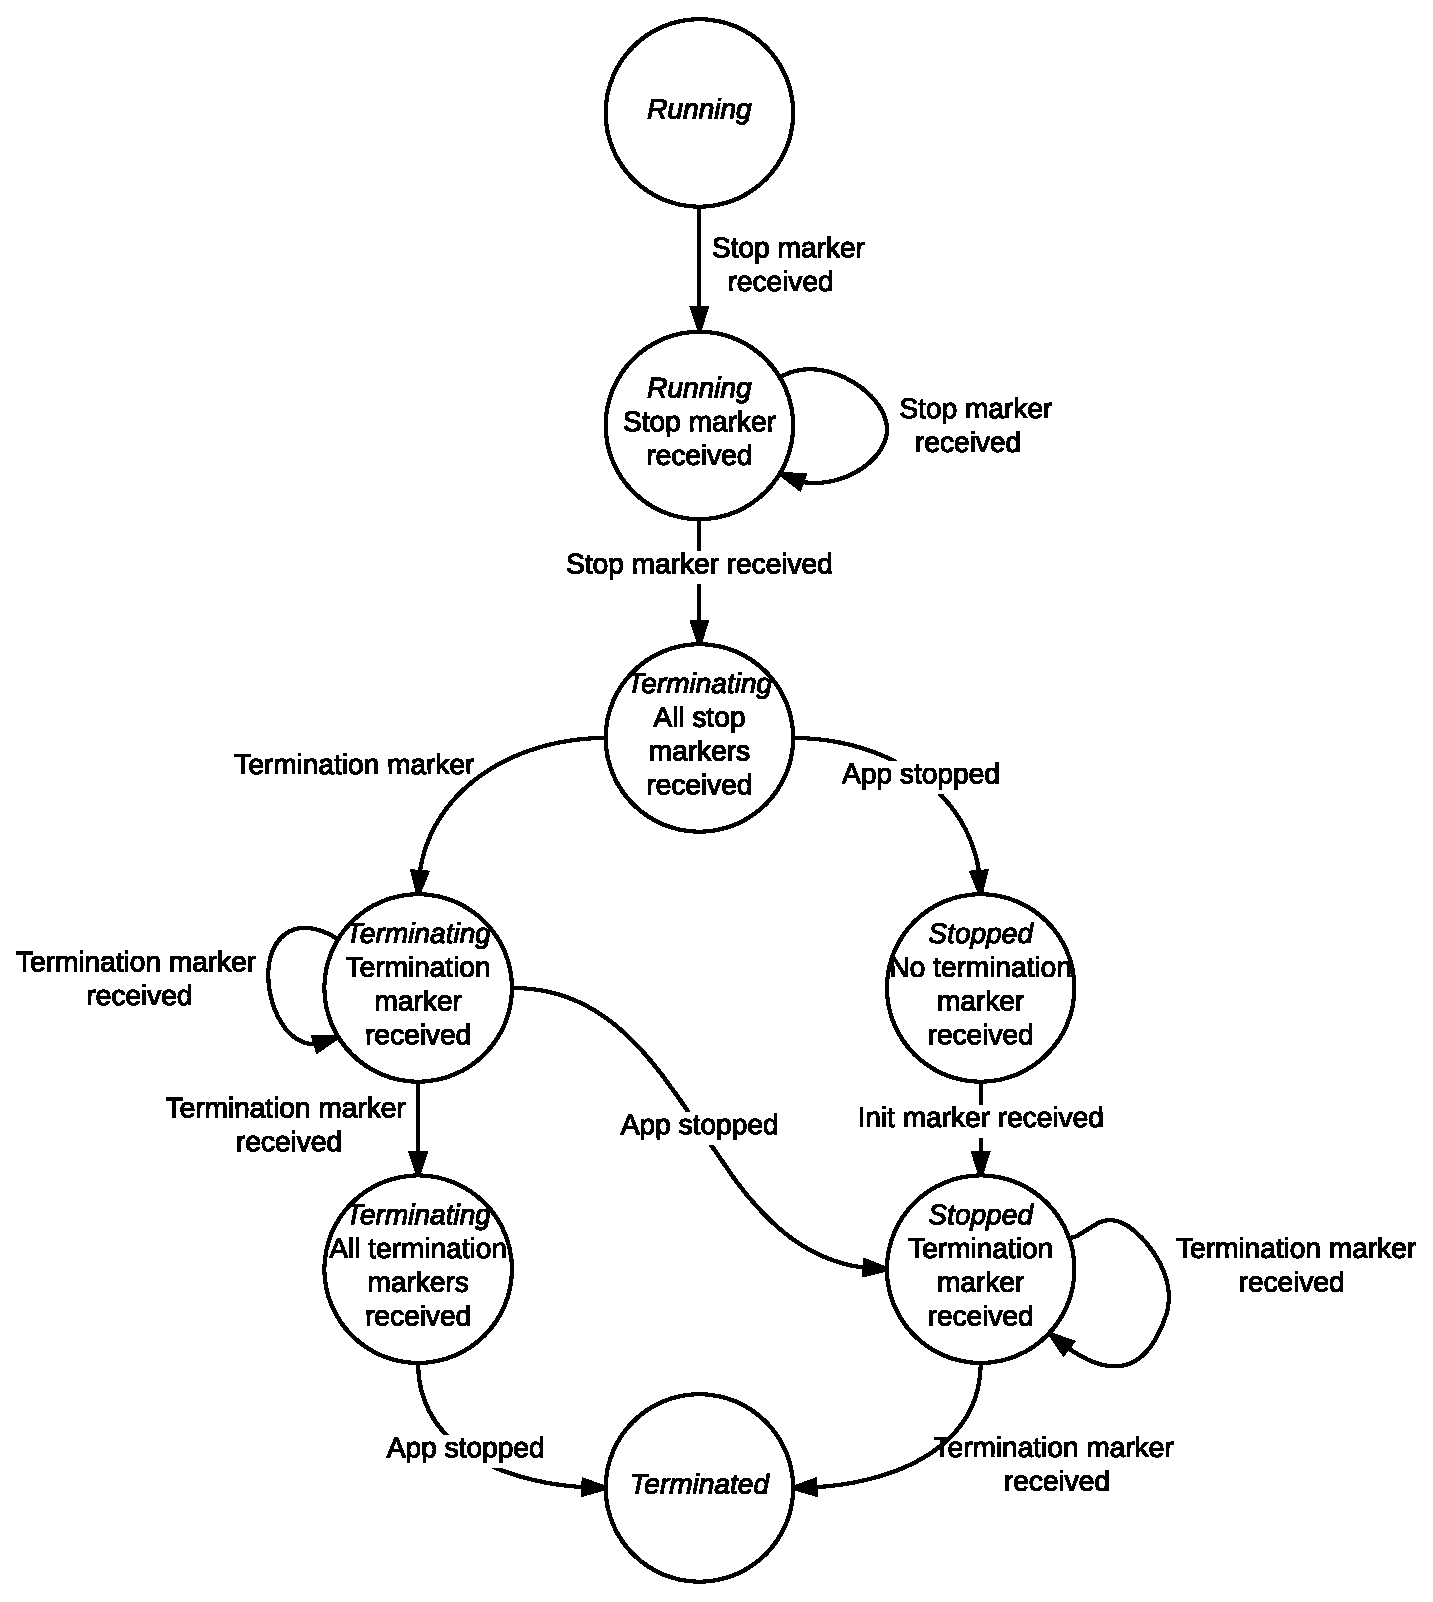
\includegraphics[width=\columnwidth]{images/solution/mw/termination.eps}
  \caption{Middleware's Termination service}
  \label{fig:mw-termination}
\end{figure}

% TODO: All class diagrams have to be added
\subsubsubsection{termination.Termination}

\begin{figure}[H]
  \centering
  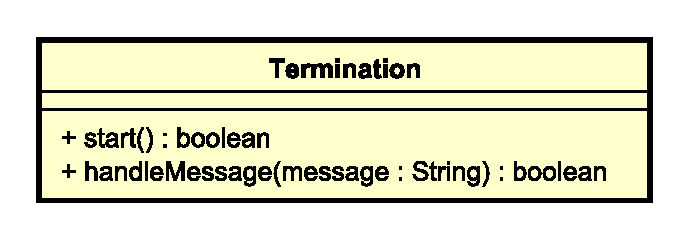
\includegraphics[width=.5\columnwidth]{images/solution/mw/ter/ter.eps}
  \caption{termination.Termination}
  \label{fig:mw-termination-termination}
\end{figure}
    % TODO: check this out: will Message actually be a String?

\FloatBarrier
\begin{itemize}
  \item \textbf{Description} \\
    This module is the Fa\c cade of the Termination service. It is responsible
    to boot neatly and supervise all processes in Termination. Also, it has to
    handle termination requests that come from other nodes of the system.
  \item \textbf{Attributes}
  \item \textbf{Operations}
  \begin{itemize}
    \item \texttt{+ start()} \\
    Starts the Termination service.
    \item \texttt{+ handleMessage(message: String)} \\
    % TODO: check this out: Message will really be a String?
    Handles a termination start/finishing request that comes from other nodes
    or receives termination information from the application layer.
  \end{itemize}
\end{itemize}

\subsubsubsection{termination.TerminationAlgorithm}

\begin{figure}[H]
  \centering
  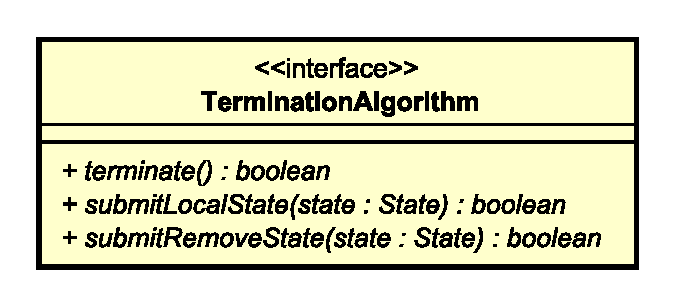
\includegraphics[width=.5\columnwidth]{images/solution/mw/ter/talg.eps}
  \caption{termination.TerminationAlgorithm}
  \label{fig:mw-termination-term-alg}
\end{figure}
    % TODO: define State type

\FloatBarrier
\begin{itemize}
  \item \textbf{Description} \\
    Interface for processes that implement a certain kind of termination.
  \item \textbf{Attributes}
  \item \textbf{Operations}
  \begin{itemize}
    \item \texttt{+ terminate()} \\
    Terminates the system.
    \item \texttt{+ submitLocalState(state : State)} \\
    Stores a final local snapshot.
    % TODO: define State type
    \item \texttt{+ submitRemoteState(state : State)} \\
    Stores a final remote snapshot.
    % TODO: define State type
  \end{itemize}
\end{itemize}

\subsubsubsection{termination.SimpleShutdown}

\begin{figure}[H]
  \centering
  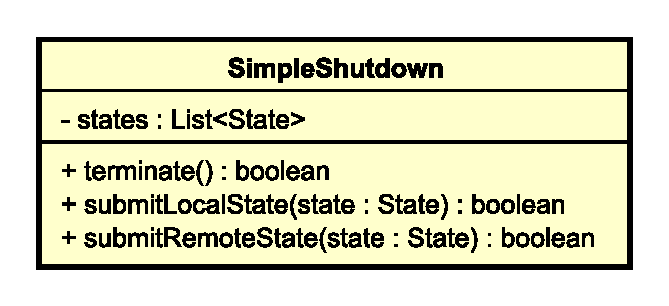
\includegraphics[width=.5\columnwidth]{images/solution/mw/ter/sshut.eps}
  \caption{termination.SimpleShutdown}
  \label{fig:mw-termination-simple-shutdown}
\end{figure}
    % TODO: define State type

\FloatBarrier
\begin{itemize}
  \item \textbf{Description} \\
    Module that implements the \texttt{termination.TerminationAlgorithm}
    interface to terminate the system with a simple algorithm.
  \item \textbf{Attributes}
  \begin{itemize}
    \item \texttt{- states : List<State>} \\
    Collection of final states.
  \end{itemize}
  \item \textbf{Operations}
  \begin{itemize}
    \item \texttt{+ terminate()} \\
    Terminates the system by requesting the application, the middleware and
    other nodes to terminate.
    \item \texttt{+ submitLocalState(state : State)} \\
    Stores the state of the local node.
    % TODO: define State type
    \item \texttt{+ submitRemoteState(state : State)} \\
    Stores the state of a remote node.
    % TODO: define State type
  \end{itemize}
\end{itemize}
